\documentclass{beamer}

\mode<presentation>
\title{SoC1\&2: Peripherals IRQ Structure}
\author[AS]{Andreas Siggelkow \newline \texttt{andreas.siggelkow@rwu.de}}
\date[2026]{\today}
\subtitle{RWU}
\institute{Elektrotechnik und Informatik}

%%%%%%%%%%%%%%%%%%%%%%%%%%%%%%%%
% Logo
%%%%%%%%%%%%%%%%%%%%%%%%%%%%%%%%
\pgfdeclareimage[height=1cm]{hslogo}{./hs}
\logo{\pgfuseimage{hslogo}}
%%%%%%%%%%%%%%%%%%%%%%%%%%%%%%%%
% Macros
%%%%%%%%%%%%%%%%%%%%%%%%%%%%%%%%
\usepackage[T1]{fontenc}
\usepackage{lmodern}
\usepackage{textcomp}
\definecolor{links}{HTML}{2A1B81}
\hypersetup{colorlinks,linkcolor=,urlcolor=links}
\usepackage{graphicx}
\usepackage{ragged2e, tabularx}
\newcolumntype{Y}{>{\RaggedRight\arraybackslash}X}
\usetheme{Singapore}
\usecolortheme{seahorse}
\usefonttheme[onlylarge]{structuresmallcapsserif}
\usefonttheme[onlysmall]{structurebold}
\setbeamertemplate{footline}[frame number]
\setbeamerfont{itemize/enumerate body}{size=\small}
\setbeamerfont{itemize/enumerate subbody}{size=\footnotesize}
\usepackage{listings}
\newcommand{\astitle}{nix}
\newcommand{\assubtitle}{nix}
\newcommand{\asfolie}[3]{\begin{frame}\frametitle{#1}\begin{block}{#2}{#3}\end{block}\end{frame}}

% Code and register access sequences are set with listings: dashes, $, _, \
% and quotes appear exactly as they have to be typed.
\definecolor{lstbg}{HTML}{F2F2F7}
\definecolor{lstcomment}{HTML}{5A5A8A}
\lstset{
  basicstyle=\ttfamily\scriptsize,
  columns=fullflexible,
  keepspaces=true,
  upquote=true,
  breaklines=true,
  breakatwhitespace=false,
  backgroundcolor=\color{lstbg},
  frame=none,
  xleftmargin=2pt,
  xrightmargin=2pt,
  aboveskip=4pt,
  belowskip=4pt,
  showstringspaces=false
}
\lstdefinestyle{sh}{
  morecomment=[l]{\#},
  commentstyle=\color{lstcomment}\itshape
}
\lstdefinestyle{c}{
  language=C,
  morecomment=[l]{//},
  commentstyle=\color{lstcomment}\itshape,
  keywordstyle=\bfseries
}
\lstdefinestyle{out}{basicstyle=\ttfamily\tiny}
\newcommand{\cmd}[1]{\texttt{#1}}

%%%%%%%%%%%%%%%%%%%%%%%%%%%%%%%%
% Register description macros (same layout as in the RWU-RV64I spec,
% latex_all_makros.tex), shrunk to slide size.
%%%%%%%%%%%%%%%%%%%%%%%%%%%%%%%%
\newcommand{\asregkopf}[2]{%
{\scriptsize
\begin{tabularx}{\textwidth}{@{}Xr@{}}
  \textbf{#1} & [Reset value: {#2}]
\end{tabularx}}\par}

\newcommand{\asregfourxsixteen}[8]{%
{\tiny\setlength{\tabcolsep}{1pt}\renewcommand{\arraystretch}{0.95}%
\begin{tabularx}{\textwidth}{|*{16}{>{\centering\arraybackslash}X|}}
  \hline
  63 & 62 & 61 & 60 & 59 & 58 & 57 & 56 & 55 & 54 & 53 & 52 & 51 & 50 & 49 & 48 \\
  \hline
  #1 \\
  \hline
  #2 \\
  \hline
  \hline
  47 & 46 & 45 & 44 & 43 & 42 & 41 & 40 & 39 & 38 & 37 & 36 & 35 & 34 & 33 & 32 \\
  \hline
  #3 \\
  \hline
  #4 \\
  \hline
  \hline
  31 & 30 & 29 & 28 & 27 & 26 & 25 & 24 & 23 & 22 & 21 & 20 & 19 & 18 & 17 & 16 \\
  \hline
  #5 \\
  \hline
  #6 \\
  \hline
  \hline
  15 & 14 & 13 & 12 & 11 & 10 & 09 & 08 & 07 & 06 & 05 & 04 & 03 & 02 & 01 & 00 \\
  \hline
  #7 \\
  \hline
  #8 \\
  \hline
\end{tabularx}}\par}

\newcommand{\asregdesc}[1]{%
{\tiny\renewcommand{\arraystretch}{1.1}%
\begin{tabularx}{\dimexpr\textwidth-1.1cm\relax}{|l|l|l|Y|}
  \hline
  \textbf{Field} & \textbf{Bits} & \textbf{Type} & \textbf{Description} \\
  \hline
  #1 \\
  \hline
\end{tabularx}}\par}

% One register field spanning all 16 bits of a row
\newcommand{\asrow}[1]{\multicolumn{16}{|c|}{#1}}

\usepackage{tikz}
\usetikzlibrary{shapes.arrows}
\usetikzlibrary{shapes.multipart}
\usetikzlibrary{positioning}
\usetikzlibrary{automata}

% Timing diagrams: a signal is a path that alternates between low (y) and
% high (y+0.4) with |- , so every waypoint is "time, level".
\newcommand{\wlabel}[2]{\node[anchor=east,font=\tiny] at (0,#1+0.2) {#2};}
\newcommand{\wgrid}[1]{\foreach \t in {0,...,#1} \draw[very thin,lightgray] (\t,-0.2) -- (\t,6.2);}

\begin{document}
%%%%%%%%%%%%%%%%%%%%%%%%%%%%%%%%
% First pages
%%%%%%%%%%%%%%%%%%%%%%%%%%%%%%%%
\setcounter{tocdepth}{1}

\begin{frame}
  \titlepage
\end{frame}

\begin{frame}
  \frametitle{Outline}
  \tableofcontents
\end{frame}

%%%%%%%%%%%%%%%%%%%%%%%%%%%%%%%%
% Introduction
%%%%%%%%%%%%%%%%%%%%%%%%%%%%%%%%
\section{Introduction}
\renewcommand{\astitle}{Introduction}
\begin{frame}
\frametitle{\astitle}
\textcolor{red}{Introduction}
\end{frame}

\renewcommand{\assubtitle}{Why an Interrupt Structure in every Peripheral?}
\begin{frame}
\frametitle{\astitle}
\begin{block}{\assubtitle}
  \begin{itemize}
    \item A peripheral kernel detects \textbf{events}: a pin changed, a byte was
      received, the TX FIFO has space, a frame error occurred, \ldots
    \item An event is only a \textbf{1-clock-cycle pulse}. Software is much slower:
      the event must be \textbf{stored} until software has handled it.
    \item Software must be able to
      \begin{itemize}
        \item find out \textbf{which} event happened,
        \item \textbf{enable/disable} single events,
        \item \textbf{acknowledge} (clear) an event,
        \item \textbf{force} an event to test the interrupt path without real hardware.
      \end{itemize}
    \item Every peripheral needs exactly this
      $\Rightarrow$ one \textbf{common register structure} for all peripherals.
  \end{itemize}
\end{block}
\end{frame}

\renewcommand{\assubtitle}{Origin: TOPSPIN Service Request Block (SRB)}
\begin{frame}
\frametitle{\astitle}
\begin{block}{\assubtitle}
  \begin{itemize}
    \item Taken from the TOPSPIN peripheral architecture concepts (2003):
      every bus peripheral contains a \textbf{Service Request Block (SRB)}.
    \item The SRB prepares the interrupt requests for the
      \textbf{Interrupt Control Unit (ICU)} and the data transfer requests
      for the DMA controller.
    \item Basic register set: \textbf{RIS, IMSC, MIS, ICR, ISR}
      (+ DMAE for DMA).
    \item Extension for an interrupt with \textbf{several sources of the same type}:
      \textbf{IRQSS, IRQSM, IRQSC}.
    \item The same register names and the same behaviour in every peripheral
      $\Rightarrow$ one driver pattern for all of them.
  \end{itemize}
\end{block}
\end{frame}

\renewcommand{\assubtitle}{What we changed for the RWU-RV64I}
\begin{frame}
\frametitle{\astitle}
\begin{block}{\assubtitle}
  \begin{itemize}
    \item \textbf{No DMA}: register DMAE and the data transfer request path are dropped.
    \item \textbf{64-bit registers}, one 8-byte aligned offset per register.
    \item One shared RTL block for all peripherals:\\
      \cmd{ip\_irqper/src/as\_irq\_peripheral.sv}, used by GPIO0, UART0 and QSPI0.
    \item \textbf{Set wins over clear}: an event in the same cycle as a clear
      is never lost.
    \item For sources of the same type, RIS[0] is \textbf{not stored again}:
      it is the level |(IRQSS \& IRQSM), so writing IRQSC is enough.
    \item ICR/ISR/IRQSC are \textbf{write strobes}, not registers: they read 0.
  \end{itemize}
\end{block}
\end{frame}

\renewcommand{\assubtitle}{Interrupt Path on Chip Level}
\begin{frame}
\frametitle{\astitle}
\begin{block}{\assubtitle}
\centering
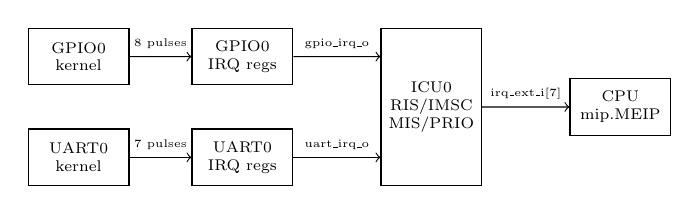
\begin{tikzpicture}[scale=0.8, transform shape,
    box/.style={draw, minimum height=0.9cm, minimum width=1.6cm, align=center, font=\scriptsize}]
  \node[box] (k1) at (0,1.2) {GPIO0\\kernel};
  \node[box] (s1) at (2.6,1.2) {GPIO0\\IRQ regs};
  \node[box] (k2) at (0,-0.4) {UART0\\kernel};
  \node[box] (s2) at (2.6,-0.4) {UART0\\IRQ regs};
  \node[box, minimum height=2.5cm] (icu) at (5.6,0.4) {ICU0\\RIS/IMSC\\MIS/PRIO};
  \node[box] (cpu) at (8.6,0.4) {CPU\\mip.MEIP};
  \draw[->] (k1) -- node[above,font=\tiny]{8 pulses} (s1);
  \draw[->] (k2) -- node[above,font=\tiny]{7 pulses} (s2);
  \draw[->] (s1) -- node[above,font=\tiny]{gpio\_irq\_o} (icu.west |- s1);
  \draw[->] (s2) -- node[above,font=\tiny]{uart\_irq\_o} (icu.west |- s2);
  \draw[->] (icu) -- node[above,font=\tiny]{irq\_ext\_i[7]} (cpu);
\end{tikzpicture}
\end{block}
  \begin{itemize}
    \item \textbf{This HowTo}: the IRQ registers inside each peripheral.
    \item ICU0 (\cmd{0x1\_0000\_0800}) collects one line per peripheral
      (source 0 = GPIO0, 1 = UART0, 2 = QSPI0) and drives the
      machine external interrupt of the CPU.
    \item \textbf{ICU0 latches the rising edge} of each peripheral line
      $\Rightarrow$ important for the IRQ flow (see later).
  \end{itemize}
\end{frame}

%%%%%%%%%%%%%%%%%%%%%%%%%%%%%%%%
% IRQ Structure
%%%%%%%%%%%%%%%%%%%%%%%%%%%%%%%%
\section{IRQ Structure}
\renewcommand{\astitle}{IRQ Structure}
\begin{frame}
\frametitle{\astitle}
\textcolor{red}{IRQ Structure}
\end{frame}

\renewcommand{\assubtitle}{The Register Set}
\begin{frame}
\frametitle{\astitle}
\begin{block}{\assubtitle}
{\scriptsize
\begin{tabularx}{\textwidth}{|l|l|l|Y|}
  \hline
  \textbf{Name} & \textbf{Mode} & \textbf{Stored} & \textbf{Function} \\
  \hline
  \hline
  RIS   & r  & yes & Raw Interrupt Status: 1 = event happened (pending) \\
  \hline
  IMSC  & rw & yes & Interrupt Mask Control: 1 = this RIS bit may raise the IRQ \\
  \hline
  MIS   & r  & no  & Masked Interrupt Status = RIS \& IMSC \\
  \hline
  ICR   & w  & no  & Interrupt Clear: writing 1 clears the RIS bit \\
  \hline
  ISR   & w  & no  & Interrupt Set: writing 1 sets the RIS bit (SW test) \\
  \hline
  \hline
  \multicolumn{4}{|l|}{\textit{only for IRQs of the same type}} \\
  \hline
  IRQSS & r  & yes & IRQ Source Status: one sticky bit per source \\
  \hline
  IRQSM & rw & yes & IRQ Source Mask: 1 = this source contributes to RIS[0] \\
  \hline
  IRQSC & w  & no  & IRQ Source Clear: writing 1 clears the IRQSS bit \\
  \hline
\end{tabularx}}
\end{block}
  \begin{itemize}
    \item All write-1 registers act bit by bit: a 0 leaves the bit unchanged.
    \item The peripheral IRQ output is \cmd{irq\_o = |MIS}.
  \end{itemize}
\end{frame}

\renewcommand{\assubtitle}{Two Cases}
\begin{frame}
\frametitle{\astitle}
\begin{block}{\assubtitle}
  \begin{itemize}
    \item \textbf{Different IRQs} (e.g.\ UART0)
      \begin{itemize}
        \item Every event has its own meaning: rx\_ready, tx\_ready, rx\_timeout,
          frame\_err, parity\_err, overrun\_err, break\_det.
        \item One RIS bit per event: \cmd{irq\_other\_i[n] -> RIS[n]}.
        \item Registers: RIS, IMSC, MIS, ICR, ISR.
      \end{itemize}
    \item \textbf{IRQs of the same type} (e.g.\ GPIO0)
      \begin{itemize}
        \item Many sources with the same meaning: ``pin $k$ changed'', $k = 0\ldots7$.
        \item One IRQSS bit per source; the sources are ORed into \textbf{one} RIS bit:
          \cmd{irq\_same\_i[k] -> IRQSS[k] -> RIS[0]}.
        \item Additional registers IRQSS, IRQSM, IRQSC.
        \item Different IRQs may exist next to the group: \cmd{irq\_other\_i[n] -> RIS[n+1]}.
      \end{itemize}
    \item Selected by parameter \cmd{irqs\_yes\_no} (0 or 1).
  \end{itemize}
\end{block}
\end{frame}

\renewcommand{\assubtitle}{Different IRQs: one Request}
\begin{frame}
\frametitle{\astitle}
\begin{block}{\assubtitle}
\begin{figure}[H]
\centering
\begin{tikzpicture}[scale=0.62, transform shape]
  % RIS
  \draw (0,0) rectangle (1,1);
  \node (RIS) at (0.5,1.25) {RIS};
  %IMSC
  \draw (0,4) rectangle (1,5);
  \node (IMSC) at (0.5,5.25) {IMSC};
  % MIS
  \draw (4,4) rectangle (5,5);
  \node (MIS) at (4.5,5.25) {MIS};
  % Mux
  \draw (-2,1.5) -- (-1,1) -- (-1,0) -- (-2,-0.5) -- (-2,1.5);
  % ISR
  \draw (-5,0) rectangle (-4,1);
  \node (ISR) at (-4.5,1.25) {ISR};
  % ICR
  \draw (-5,-2) rectangle (-4,-1);
  \node (ICR) at (-4.5,-0.75) {ICR};
  % AND
  \draw (2,2) rectangle (3,3);
  \node (AND) at (2.5,2.25) {\&};
  % Lines
  \draw[->] (-4,0.5) -- (-2,0.5); % ISR to Mux
  \draw (-4,-1.5) -- (-3,-1.5); % ICR to Mux (1)
  \draw (-3,-1.5) -- (-3,0); % ICR to Mux (2)
  \draw[->] (-3,0) -- (-2,0); % ICR to Mux (3)
  \draw (-4,2.5) -- (-3,2.5); % IRQ to Mux (1)
  \draw (-3,2.5) -- (-3,1); % IRQ to Mux (2)
  \draw[->] (-3,1) -- (-2,1); % IRQ to Mux (3)
  \draw[->] (-1,0.5) -- (0,0.5); % Mux to RIS
  \draw (1,0.5) -- (1.5,0.5); % RIS to AND (1)
  \draw (1.5,0.5) -- (1.5,2.25); % RIS to AND (2)
  \draw[->] (1.5,2.25) -- (2,2.25); % RIS to AND (3)
  \draw (1,4.5) -- (1.5,4.5); % IMSC to AND (1)
  \draw (1.5,4.5) -- (1.5,2.75); % IMSC to AND (2)
  \draw[->] (1.5,2.75) -- (2,2.75); % IMSC to AND (3)
  \draw[->] (3,2.5) -- (5,2.5); % AND to output
  \draw (3.5, 2.5) -- (3.5,4.5); %AND to MIS
  \draw[->] (3.5,4.5) -- (4,4.5); %AND to MIS
  % more Nodes
  \node (IRQ1) at (-5,2.5) {IRQ Src};
  \node (IRQ2) at (6.5,2.5) {IRQ to ICU};
  % Soldering dot
  \fill [black] (3.5,2.5) circle (0.1);

\end{tikzpicture}
\caption{Interrupt Request Flow (one bit $n$)}
\label{fig:irqflow01}
\end{figure}
\end{block}
\end{frame}

\renewcommand{\assubtitle}{Different IRQs: how it works}
\begin{frame}[fragile]
\frametitle{\astitle}
\begin{block}{\assubtitle}
  \begin{itemize}
    \item A pulse on \cmd{irq\_other\_i[n]} sets RIS[$n$].
    \item RIS[$n$] is \textbf{sticky}: it stays 1 until software writes a 1 to ICR[$n$].
    \item Software can set RIS[$n$] by writing a 1 to ISR[$n$].
    \item IMSC[$n$] decides whether RIS[$n$] reaches MIS[$n$] and the IRQ output.
    \item All bits of MIS are ORed: one IRQ line per peripheral to ICU0.
  \end{itemize}
\end{block}
\begin{block}{RTL (as\_irq\_peripheral.sv)}
\begin{lstlisting}
ris_r <= (ris_r & ~ris_clr_s) | ris_set_s;  // set wins over clear
assign mis_s = ris_s & imsc_r;
assign irq_o = |mis_s;
\end{lstlisting}
\end{block}
\end{frame}

\renewcommand{\assubtitle}{IRQs of the same Type: Source Registers}
\begin{frame}
\frametitle{\astitle}
\begin{block}{\assubtitle}
\begin{figure}[H]
\centering
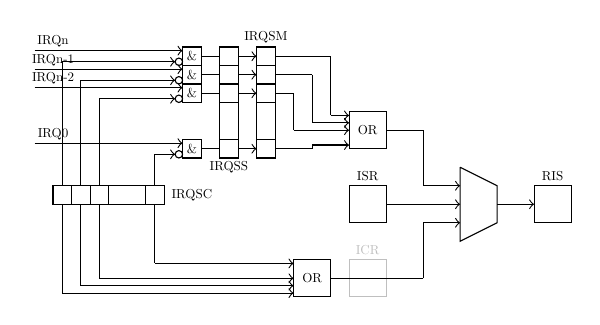
\begin{tikzpicture}[scale=0.47, transform shape]
  % RIS
  \draw (0,0) rectangle (1,1);
  \node (RIS) at (0.5,1.25) {RIS};
  % Mux
  \draw (-2,1.5) -- (-1,1) -- (-1,0) -- (-2,-0.5) -- (-2,1.5);
  % ISR
  \draw (-5,0) rectangle (-4,1);
  \node (ISR) at (-4.5,1.25) {ISR};
  % ICR
  \draw[draw=lightgray] (-5,-2) rectangle (-4,-1);
  \node[text=lightgray] (ICR) at (-4.5,-0.75) {ICR};
  % OR1
  \draw (-5,2) rectangle (-4,3);
  \node (OR1) at (-4.5,2.5) {OR};
  % OR2
  \draw (-6.5,-2) rectangle (-5.5,-1);
  \node (OR2) at (-6,-1.5) {OR};
  % IRQSM
  \draw (-7.5,1.75) rectangle (-7,2.25); % small lower
  \draw (-7.5,2.25) rectangle (-7,3.25); % the dots rectangle
  \draw (-7.5,3.25) rectangle (-7,3.75); % small upper
  \draw (-7.5,3.75) rectangle (-7,4.25); % small upper
  \draw (-7.5,4.25) rectangle (-7,4.75); % small highest
  % IRQSS
  \draw (-8.5,1.75) rectangle (-8,2.25); % small lower
  \draw (-8.5,2.25) rectangle (-8,3.25); % the dots rectangle
  \draw (-8.5,3.25) rectangle (-8,3.75); % small upper
  \draw (-8.5,3.75) rectangle (-8,4.25); % small upper
  \draw (-8.5,4.25) rectangle (-8,4.75); % small highest
  % IRQSC
  \draw (-10.5,0.5) rectangle (-10,1); % small right
  \draw (-11.5,0.5) rectangle (-10.5,1); % the dots rectangle
  \draw (-12,0.5) rectangle (-11.5,1); % small
  \draw (-12.5,0.5) rectangle (-12,1); % small
  \draw (-13,0.5) rectangle (-12.5,1); % small left
  % small ANDs with inverter circle at input 1
  % AND1
  \draw (-9.5,1.75) rectangle (-9,2.25);
  \node (AND1) at (-9.25,2.0) {\&};
  \draw (-9.6,1.85) circle (0.1);
  % AND2
  \draw (-9.5,3.25) rectangle (-9,3.75);
  \node (AND2) at (-9.25,3.5) {\&};
  \draw (-9.6,3.35) circle (0.1);
  % AND3
  \draw (-9.5,3.75) rectangle (-9,4.25);
  \node (AND3) at (-9.25,4) {\&};
  \draw (-9.6,3.85) circle (0.1);
  % AND3
  \draw (-9.5,4.25) rectangle (-9,4.75);
  \node (AND3) at (-9.25,4.5) {\&};
  \draw (-9.6,4.35) circle (0.1);
  % Lines
  \draw[->] (-4,0.5) -- (-2,0.5); % ISR to Mux
  \draw (-4,-1.5) -- (-3,-1.5); % ICR to Mux (1)
  \draw (-3,-1.5) -- (-3,0); % ICR to Mux (2)
  \draw[->] (-3,0) -- (-2,0); % ICR to Mux (3)
  \draw (-4,2.5) -- (-3,2.5); % IRQ to Mux (1)
  \draw (-3,2.5) -- (-3,1); % IRQ to Mux (2)
  \draw[->] (-3,1) -- (-2,1); % IRQ to Mux (3)
  \draw[->] (-1,0.5) -- (0,0.5); % Mux to RIS
  \draw (-7,2) -- (-6,2); %IRQSM to OR (1)
  \draw (-6,2) -- (-6,2.1); %IRQSM to OR (1)
  \draw[->] (-6,2.1) -- (-5,2.1); % IRQSM to OR (1)
  \draw (-7,3.5) -- (-6.5,3.5); % IRQSM to OR (2)
  \draw (-6.5,3.5) -- (-6.5,2.5); % IRQSM to OR (2)
  \draw[->] (-6.5,2.5) -- (-5,2.5); % IRQSM to OR (2)
  \draw (-7,4.0) -- (-6.0,4.0); % IRQSM to OR (3)
  \draw (-6.0,4.0) -- (-6.0,2.7); % IRQSM to OR (3)
  \draw[->] (-6.0,2.7) -- (-5,2.7); % IRQSM to OR (3)
  \draw (-7,4.5) -- (-5.5,4.5); % IRQSM to OR (4)
  \draw (-5.5,4.5) -- (-5.5,2.9); % IRQSM to OR (4)
  \draw[->] (-5.5,2.9) -- (-5,2.9); % IRQSM to OR (4)
  \draw (-5.5,-1.5) -- (-3.0,-1.5); % OR to Mux
  \draw[->] (-8,2) -- (-7.5,2); % IRQSS to IRQSM
  \draw[->] (-8,3.5) -- (-7.5,3.5); % IRQSS to IRQSM
  \draw[->] (-8,4.0) -- (-7.5,4.0); % IRQSS to IRQSM
  \draw[->] (-8,4.5) -- (-7.5,4.5); % IRQSS to IRQSM
  \draw (-9,2) -- (-8.5,2); % Little AND to IRQSS
  \draw (-9,3.5) -- (-8.5,3.5); % Little AND to IRQSS
  \draw (-9,4.0) -- (-8.5,4.0); % Little AND to IRQSS
  \draw (-9,4.5) -- (-8.5,4.5); % Little AND to IRQSS
  \draw[->] (-13.5,2.15) -- (-9.5,2.15); % IRQ to little AND
  \draw[->] (-13.5,3.65) -- (-9.5,3.65); % IRQ to little AND
  \draw[->] (-13.5,4.15) -- (-9.5,4.15); % IRQ to little AND
  \draw[->] (-13.5,4.65) -- (-9.5,4.65); % IRQ to little AND
  \draw (-10.25,1.00) -- (-10.25,1.85); % IRQSC to little AND
  \draw[->] (-10.25,1.85) -- (-9.7,1.85); % IRQSC to little AND
  \draw (-11.75,1.00) -- (-11.75,3.35); % IRQSC to little AND
  \draw[->] (-11.75,3.35) -- (-9.7,3.35); % IRQSC to little AND
  \draw (-12.25,1.00) -- (-12.25,3.85); % IRQSC to little AND
  \draw[->] (-12.25,3.85) -- (-9.7,3.85); % IRQSC to little AND
  \draw (-12.75,1.00) -- (-12.75,4.35); % IRQSC to little AND
  \draw[->] (-12.75,4.35) -- (-9.7,4.35); % IRQSC to little AND
  \draw        (-10.25,0.50) -- (-10.25,-1.10); % IRQSC to OR
  \draw[->] (-10.25,-1.10) -- (-6.50,-1.10); % IRQSC to OR
  \draw        (-11.75,0.50) -- (-11.75,-1.50); % IRQSC to OR
  \draw[->] (-11.75,-1.50) -- (-6.50,-1.50); % IRQSC to OR
  \draw        (-12.25,0.50) -- (-12.25,-1.70); % IRQSC to OR
  \draw[->] (-12.25,-1.70) -- (-6.50,-1.70); % IRQSC to OR
  \draw        (-12.75,0.50) -- (-12.75,-1.90); % IRQSC to OR
  \draw[->] (-12.75,-1.90) -- (-6.50,-1.90); % IRQSC to OR

  % more Nodes
  \node (IRQ0) at (-13.0,2.15+0.25) {IRQ0};
  \node (IRQn2) at (-13.0,3.65+0.25) {IRQn-2};
  \node (IRQn1) at (-13.0,4.15+0.25) {IRQn-1};
  \node (IRQn) at (-13.0,4.65+0.25) {IRQn};

  \node (IRQSM) at (-7.25,4.75+0.25) {IRQSM};
  \node (IRQSS) at (-8.25,1.5) {IRQSS};
  \node (IRQSC) at (-9.25,0.75) {IRQSC};

\end{tikzpicture}
\caption{Interrupt Request with multiple sources (TOPSPIN)}
\label{fig:irqflow02}
\end{figure}
\end{block}
\end{frame}

\renewcommand{\assubtitle}{IRQs of the same Type: how it works}
\begin{frame}
\frametitle{\astitle}
\begin{block}{\assubtitle}
  \begin{itemize}
    \item A pulse on source $k$ sets IRQSS[$k$] (sticky).
    \item IRQSM[$k$] masks source $k$ \textbf{before} the OR.
    \item The OR of all unmasked pending sources forms the group request in RIS[0].
    \item IRQSC replaces ICR: writing 1 to IRQSC[$k$] clears IRQSS[$k$].
    \item TOPSPIN: an ISR-forced RIS bit is cleared by \textbf{any} IRQSC bit
      (OR into the grey ICR path).
  \end{itemize}
\end{block}
\begin{block}{RWU-RV64I implementation (simpler)}
  \begin{itemize}
    \item RIS[0] = |(IRQSS \& IRQSM) | ris\_r[0]: no second flip-flop.
    \item IRQSC alone clears the group; ICR[0] only an ISR-forced bit 0.
  \end{itemize}
\end{block}
\end{frame}

\renewcommand{\assubtitle}{Signal Flow of as\_irq\_peripheral (irqs\_yes\_no = 1)}
\begin{frame}[fragile]
\frametitle{\astitle}
\begin{block}{\assubtitle}
\begin{lstlisting}
  irq_same_i --> IRQSS --&--> OR --+
                 IRQSM --'         |
                                   v
  irq_other_i -------------------> RIS --&--> MIS --> OR --> irq_o
  ISR (write 1 = set) -----------> RIS    |
  ICR (write 1 = clear) ---------> RIS  IMSC
\end{lstlisting}
\end{block}
\begin{block}{RTL}
\begin{lstlisting}
irqss_r <= (irqss_r & ~(wr_irqsc_s ? data_i : '0)) | irq_same_i;
assign irq_same_comb_s = |(irqss_r & irqsm_r);
assign ris_s = ris_r | {{(data_width-1){1'b0}}, irq_same_comb_s};
\end{lstlisting}
\end{block}
  \begin{itemize}
    \item With \cmd{irqs\_yes\_no = 0} IRQSS/IRQSM/IRQSC are not built
      (generate), their offsets are not decoded.
  \end{itemize}
\end{frame}

\renewcommand{\assubtitle}{Parameters of as\_irq\_peripheral}
\begin{frame}
\frametitle{\astitle}
\begin{block}{\assubtitle}
{\scriptsize
\begin{tabularx}{\textwidth}{|l|Y|l|l|l|}
  \hline
  \textbf{Parameter} & \textbf{Meaning} & \textbf{GPIO0} & \textbf{UART0} & \textbf{QSPI0} \\
  \hline
  \hline
  irqs\_yes\_no   & 1: IRQSS/IRQSM/IRQSC exist & 1 & 0 & 0 \\
  \hline
  nr\_same\_irqs  & number of sources of the same type (IRQSS bits) & 8 & 1 (unused) & 1 (unused) \\
  \hline
  nr\_other\_irqs & number of different IRQs (RIS bits) & 1 (tied 0) & 7 & 5 \\
  \hline
  reg\_imsc\_rst  & reset value of IMSC & all 1 & 0 & 0 \\
  \hline
  reg\_irqsm\_rst & reset value of IRQSM & all 1 & -- & -- \\
  \hline
  addr\_offs\_*   & offset of each register in the peripheral & 0x18\ldots & 0x40\ldots & 0x40\ldots \\
  \hline
\end{tabularx}}
\end{block}
  \begin{itemize}
    \item Events: \cmd{irq\_other\_i}, \cmd{irq\_same\_i} (1-cycle pulses);
      the kernel decides what an event is.
    \item ISR sets only implemented RIS bits; all others read 0.
    \item GPIO IMSC reset all 1 is temporary (``change to 0 before tape-out'').
  \end{itemize}
\end{frame}

%%%%%%%%%%%%%%%%%%%%%%%%%%%%%%%%
% IRQ Flow
%%%%%%%%%%%%%%%%%%%%%%%%%%%%%%%%
\section{IRQ Flow}
\renewcommand{\astitle}{IRQ Flow}
\begin{frame}
\frametitle{\astitle}
\textcolor{red}{IRQ Flow}
\end{frame}

\renewcommand{\assubtitle}{Different IRQs: Rules (TOPSPIN)}
\begin{frame}
\frametitle{\astitle}
\begin{block}{\assubtitle}
  \begin{itemize}
    \item An event sets its RIS bit, \textbf{independent of IMSC}.
    \item IMSC disabled while the interrupt is active: the IRQ to the ICU is
      removed, but comes back when IMSC is enabled again, unless RIS was cleared
      in the meantime.
    \item IMSC not enabled when the event occurs: only RIS is set. Enabling IMSC
      later makes the interrupt active in MIS immediately.
    \item \textbf{Good practice}: before enabling an interrupt in IMSC, first clear
      the old RIS bit via ICR.
    \item RWU-RV64I addition: event and ICR write on the same bit in the same
      cycle $\Rightarrow$ \textbf{the bit stays set}.
  \end{itemize}
\end{block}
\end{frame}

\renewcommand{\assubtitle}{Different IRQs: Timing (one RIS bit)}
\begin{frame}
\frametitle{\astitle}
\begin{block}{\assubtitle}
\centering
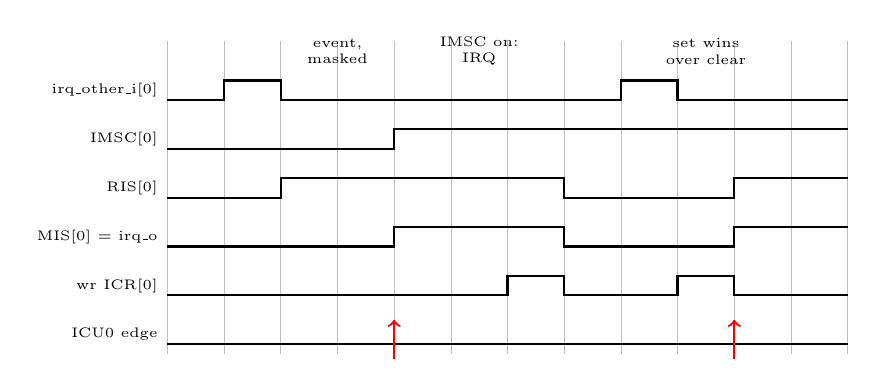
\begin{tikzpicture}[xscale=0.72, yscale=0.62]
  \wgrid{12}
  \wlabel{5}{irq\_other\_i[0]}
  \draw[thick] (0,5) -- (1,5) |- (2,5.4) |- (8,5) |- (9,5.4) |- (10,5) -- (12,5);
  \wlabel{4}{IMSC[0]}
  \draw[thick] (0,4) -- (4,4) |- (12,4.4);
  \wlabel{3}{RIS[0]}
  \draw[thick] (0,3) -- (2,3) |- (7,3.4) |- (10,3) |- (12,3.4);
  \wlabel{2}{MIS[0] = irq\_o}
  \draw[thick] (0,2) -- (4,2) |- (7,2.4) |- (10,2) |- (12,2.4);
  \wlabel{1}{wr ICR[0]}
  \draw[thick] (0,1) -- (6,1) |- (7,1.4) |- (9,1) |- (10,1.4) |- (12,1);
  \wlabel{0}{ICU0 edge}
  \draw[thick] (0,0) -- (12,0);
  \foreach \t in {4,10} \draw[->,red,thick] (\t,-0.3) -- (\t,0.5);
  \node[font=\tiny,align=center] at (3,6.0) {event,\\masked};
  \node[font=\tiny,align=center] at (5.5,6.0) {IMSC on:\\IRQ};
  \node[font=\tiny,align=center] at (9.5,6.0) {set wins\\over clear};
\end{tikzpicture}
\end{block}
  \begin{itemize}
    \item Cycle 9: new event and ICR write in the same cycle: RIS stays 1,
      the second interrupt is not lost.
  \end{itemize}
\end{frame}

\renewcommand{\assubtitle}{Different IRQs: Initialisation (UART0)}
\begin{frame}[fragile]
\frametitle{\astitle}
\begin{block}{\assubtitle}
\begin{lstlisting}[style=c]
#define UART0      0x100000600UL
#define UART0_RIS  (*(volatile uint64_t *)(UART0 + 0x40))
#define UART0_IMSC (*(volatile uint64_t *)(UART0 + 0x48))
#define UART0_MIS  (*(volatile uint64_t *)(UART0 + 0x50))
#define UART0_ICR  (*(volatile uint64_t *)(UART0 + 0x58))
#define UART0_ISR  (*(volatile uint64_t *)(UART0 + 0x60))

#define RX_READY   (1UL << 0)
#define RX_TIMEOUT (1UL << 2)
#define ERR_ALL    (0xFUL << 3)   // frame, parity, overrun, break

UART0_ICR  = 0x7F;                            // 1. clear old events
UART0_IMSC = RX_READY | RX_TIMEOUT | ERR_ALL;  // 2. enable wanted ones
// 3. ICU0_IMSC bit 1, ICU0_CTRL.GIE,
//    mie.MEIE, mstatus.MIE
\end{lstlisting}
\end{block}
\end{frame}

\renewcommand{\assubtitle}{Different IRQs: Service Routine (UART0)}
\begin{frame}[fragile]
\frametitle{\astitle}
\begin{block}{\assubtitle}
\begin{lstlisting}[style=c]
void uart0_isr(void)
{
  uint64_t mis;
  ICU0_ICR = 1UL << 1;              // 0. ack ICU0 first
  while ((mis = UART0_MIS) != 0) {  // 1. which events?
    if (mis & (RX_READY | RX_TIMEOUT))
      read_rx_fifo();               // 2. read until empty
    if (mis & ERR_ALL)
      count_errors(mis);
    UART0_ICR = mis;                // 3. clear handled bits
  }
}
\end{lstlisting}
\end{block}
  \begin{itemize}
    \item Clear only the bits you read: a new event stays pending.
    \item Loop until MIS = 0, else ICU0 never sees a new rising edge.
    \item Ack ICU0\_ICR (\cmd{0x1\_0000\_0820}) \textbf{before} the loop,
      so a later edge is not lost.
  \end{itemize}
\end{frame}

\renewcommand{\assubtitle}{Events derived from a Level}
\begin{frame}
\frametitle{\astitle}
\begin{block}{\assubtitle}
  \begin{itemize}
    \item Some events are conditions that last (UART0: rx\_ready, tx\_ready,
      rx\_timeout; QSPI0: all five sources).
    \item The kernel makes a pulse on the \textbf{rising edge} of the condition:
      RIS is set once per edge. While the condition stays true, clearing RIS
      creates \textbf{no new event}.
    \item rx\_ready: read the RX FIFO \textbf{below RXTHRES} (best: until empty),
      otherwise only rx\_timeout fires later.
    \item tx\_ready: fill the TX FIFO to RXTHRES or more, so that the next
      fall below the threshold is a new event.
    \item tx\_ready is set right after reset (TX FIFO empty)
      $\Rightarrow$ init clears RIS via ICR before enabling IMSC.
  \end{itemize}
\end{block}
\end{frame}

\renewcommand{\assubtitle}{IRQs of the same Type: Rules}
\begin{frame}
\frametitle{\astitle}
\begin{block}{\assubtitle}
  \begin{itemize}
    \item A pulse on a source sets its IRQSS bit, \textbf{independent of IRQSM}.
    \item IRQSM selects which sources form the group request;
      IMSC[0] enables the group as a whole.
    \item TOPSPIN: after reset \textbf{all sources are enabled} (IRQSM = all 1).
    \item The group request (RIS[0]) is a \textbf{level}: it stays 1 as long as at
      least one unmasked IRQSS bit is 1.
    \item Clearing: write 1s to IRQSC for the handled sources. ICR is not needed
      (only for a bit 0 forced via ISR).
    \item Event and IRQSC write on the same bit in the same cycle
      $\Rightarrow$ the IRQSS bit stays set.
  \end{itemize}
\end{block}
\end{frame}

\renewcommand{\assubtitle}{IRQs of the same Type: Timing (GPIO0)}
\begin{frame}
\frametitle{\astitle}
\begin{block}{\assubtitle}
\centering
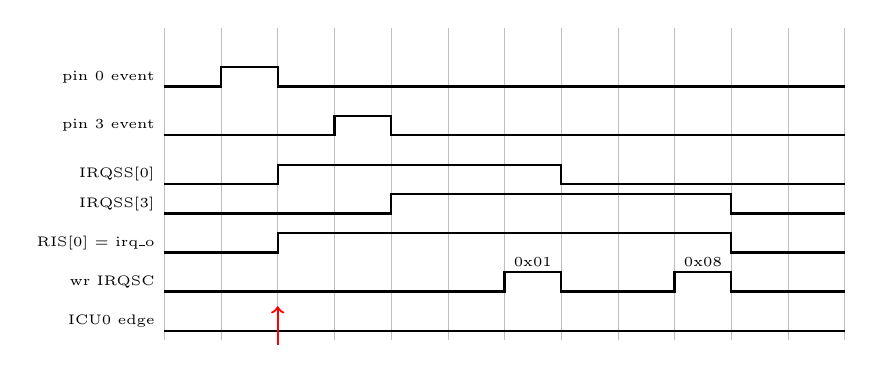
\begin{tikzpicture}[xscale=0.72, yscale=0.62]
  \wgrid{12}
  \wlabel{5}{pin 0 event}
  \draw[thick] (0,5) -- (1,5) |- (2,5.4) |- (12,5);
  \wlabel{4}{pin 3 event}
  \draw[thick] (0,4) -- (3,4) |- (4,4.4) |- (12,4);
  \wlabel{3}{IRQSS[0]}
  \draw[thick] (0,3) -- (2,3) |- (7,3.4) |- (12,3);
  \wlabel{2.4}{IRQSS[3]}
  \draw[thick] (0,2.4) -- (4,2.4) |- (10,2.8) |- (12,2.4);
  \wlabel{1.6}{RIS[0] = irq\_o}
  \draw[thick] (0,1.6) -- (2,1.6) |- (10,2.0) |- (12,1.6);
  \wlabel{0.8}{wr IRQSC}
  \draw[thick] (0,0.8) -- (6,0.8) |- (7,1.2) |- (9,0.8) |- (10,1.2) |- (12,0.8);
  \node[font=\tiny] at (6.5,1.4) {0x01};
  \node[font=\tiny] at (9.5,1.4) {0x08};
  \wlabel{0}{ICU0 edge}
  \draw[thick] (0,0) -- (12,0);
  \draw[->,red,thick] (2,-0.3) -- (2,0.5);
\end{tikzpicture}
\end{block}
  \begin{itemize}
    \item Pin 3 arrives while pin 0 is pending: \textbf{no new edge} at ICU0.
    \item After IRQSC = 0x01 the line is still high (pin 3) $\Rightarrow$
      the ISR must clear \textbf{all} pending sources.
  \end{itemize}
\end{frame}

\renewcommand{\assubtitle}{IRQs of the same Type: Service Routine (GPIO0)}
\begin{frame}[fragile]
\frametitle{\astitle}
\begin{block}{\assubtitle}
\begin{lstlisting}[style=c]
#define GPIO0       0x100000000UL
#define GPIO0_IRQSS (*(volatile uint64_t *)(GPIO0 + 0x18))
#define GPIO0_IRQSM (*(volatile uint64_t *)(GPIO0 + 0x20))
#define GPIO0_IRQSC (*(volatile uint64_t *)(GPIO0 + 0x28))
#define GPIO0_MIS   (*(volatile uint64_t *)(GPIO0 + 0x48))
void gpio0_isr(void)
{
  uint64_t pins;
  ICU0_ICR = 1UL << 0;                // 0. ack ICU0 first
  while (GPIO0_MIS & 1) {             //    group active?
    pins = GPIO0_IRQSS & GPIO0_IRQSM; // 1. which pins?
    handle_pins(pins);                // 2. handle them
    GPIO0_IRQSC = pins;               // 3. clear sources
  }
}
\end{lstlisting}
\end{block}
  \begin{itemize}
    \item Init: \cmd{GPIO0\_IRQSC = 0xFF}, select pins in \cmd{GPIO0\_IRQSM},
      then \cmd{GPIO0\_IMSC = 1}.
  \end{itemize}
\end{frame}

\renewcommand{\assubtitle}{Comparison of both Cases}
\begin{frame}
\frametitle{\astitle}
\begin{block}{\assubtitle}
{\scriptsize
\begin{tabularx}{\textwidth}{|l|Y|Y|}
  \hline
   & \textbf{Different IRQs (UART0)} & \textbf{Same type (GPIO0)} \\
  \hline
  \hline
  Event stored in & RIS[$n$] & IRQSS[$k$] \\
  \hline
  Mask & IMSC[$n$] & IRQSM[$k$], then IMSC[0] \\
  \hline
  Which event? & read MIS & read IRQSS \& IRQSM \\
  \hline
  Clear & ICR[$n$] & IRQSC[$k$] \\
  \hline
  SW test & ISR[$n$] & ISR[0], clear with ICR[0] \\
  \hline
  RIS bit & sticky flip-flop & level |(IRQSS \& IRQSM) \\
  \hline
  ISR exit & loop until MIS = 0 & loop until MIS[0] = 0 \\
  \hline
\end{tabularx}}
\end{block}
\end{frame}

%%%%%%%%%%%%%%%%%%%%%%%%%%%%%%%%
% Register Description
%%%%%%%%%%%%%%%%%%%%%%%%%%%%%%%%
\section{Register Description}
\renewcommand{\astitle}{Register Description}
\begin{frame}
\frametitle{\astitle}
\textcolor{red}{Register Description}
\end{frame}

\renewcommand{\assubtitle}{Conventions}
\begin{frame}
\frametitle{\astitle}
\begin{block}{Read-Write Features (as in the spec)}
  \begin{itemize}
    \item w: writable bit, by SW
    \item r: readable bit, by SW
    \item h: bit will be set by HW only
  \end{itemize}
\end{block}
\begin{block}{Parameters (as in TOPSPIN)}
  \begin{itemize}
    \item \cmd{nr\_of\_irq}: number of RIS bits of the peripheral
      (UART0: 7, QSPI0: 5, GPIO0: 2, i.e.\ group bit 0 + bit 1 for ISR only)
    \item \cmd{nr\_of\_irqs}: number of sources of the same type (GPIO0: 8)
    \item All registers are 64 bit wide, unused bits read 0.
  \end{itemize}
\end{block}
\end{frame}

\renewcommand{\assubtitle}{Register Overview and Offsets}
\begin{frame}
\frametitle{\astitle}
\begin{block}{\assubtitle}
{\scriptsize
\begin{tabularx}{\textwidth}{|l|Y|l|l|l|l|}
  \hline
  \textbf{Symbol} & \textbf{Register Name} & \textbf{Mode} & \textbf{GPIO0} & \textbf{UART0} & \textbf{QSPI0} \\
  \hline
  \hline
  IRQSS & Interrupt Request Source Status & rh & 0x18 & -- & -- \\
  \hline
  IRQSM & Interrupt Request Source Mask   & rw & 0x20 & -- & -- \\
  \hline
  IRQSC & Interrupt Request Source Clear  & w  & 0x28 & -- & -- \\
  \hline
  ISR   & Interrupt Set                   & w  & 0x30 & 0x60 & 0x40 \\
  \hline
  RIS   & Raw Interrupt Status            & rh & 0x38 & 0x40 & 0x48 \\
  \hline
  IMSC  & Interrupt Mask Control          & rw & 0x40 & 0x48 & 0x50 \\
  \hline
  MIS   & Masked Interrupt Status         & rh & 0x48 & 0x50 & 0x58 \\
  \hline
  ICR   & Interrupt Clear                 & w  & 0x50 & 0x58 & 0x60 \\
  \hline
\end{tabularx}}
\end{block}
  \begin{itemize}
    \item Base: GPIO0 \cmd{0x1\_0000\_0000}, QSPI0 \cmd{0x1\_0000\_0200}, UART0 \cmd{0x1\_0000\_0600}.
    \item Chip names: \textbf{GPIO0\_RIS}, \textbf{UART0\_IMSC}, \ldots
  \end{itemize}
\end{frame}

% ---------------- RIS
\renewcommand{\assubtitle}{RIS -- Raw Interrupt Status Register}
\begin{frame}
\frametitle{\astitle}
\begin{block}{\assubtitle}
{\tiny Read-only. On a read it gives the current raw status of each interrupt,
independent of IMSC. Set by an event or by ISR, cleared by ICR. A write has no effect.}
\vspace{2pt}
\asregkopf{Raw Interrupt Status Register}{$0000000000000000_H$}
\asregfourxsixteen{\asrow{0}}{\asrow{r}}
                  {\asrow{0}}{\asrow{r}}
                  {\asrow{0}}{\asrow{r}}
                  {\multicolumn{16}{|c|}{0 / RIS}}{\multicolumn{16}{|c|}{r / rh}}
\vspace{2pt}
\asregdesc{RIS & nr\_of\_irq-1:0 & rh & One status bit per service request. 0: no interrupt, 1: interrupt pending. GPIO0: bit 0 = |(IRQSS \& IRQSM) or ISR-forced; bit 1 ISR-forced only. \\
           \hline
           0 & 63:nr\_of\_irq & r & Unimplemented, reserved}
\end{block}
\end{frame}

\renewcommand{\assubtitle}{RIS -- Bit Fields of UART0\_RIS}
\begin{frame}
\frametitle{\astitle}
\begin{block}{\assubtitle}
\asregkopf{UART0\_RIS (offset 0x40)}{$0000000000000000_H$}
\asregfourxsixteen{\asrow{0}}{\asrow{r}}
                  {\asrow{0}}{\asrow{r}}
                  {\asrow{0}}{\asrow{r}}
                  {0&0&0&0&0&0&0&0&0&BD&OE&PE&FE&RT&TR&RR}
                  {r&r&r&r&r&r&r&r&r&rh&rh&rh&rh&rh&rh&rh}
\vspace{2pt}
\asregdesc{RR & 0 & rh & RX\_READY: RX FIFO level $\geq$ RXTHRES \\
           \hline
           TR & 1 & rh & TX\_READY: TX FIFO level $<$ RXTHRES (space available) \\
           \hline
           RT & 2 & rh & RX\_TIMEOUT: data in RX FIFO, no new byte for $\geq$ 4 character times \\
           \hline
           FE, PE & 3, 4 & rh & FRAME\_ERR, PARITY\_ERR (mirrored in STATUS[4], STATUS[5]) \\
           \hline
           OE, BD & 5, 6 & rh & OVERRUN\_ERR, BREAK\_DET (mirrored in STATUS[6], STATUS[7]) \\
           \hline
           - & 63:7 & r & Reserved}
\end{block}
\end{frame}

% ---------------- IMSC
\renewcommand{\assubtitle}{IMSC -- Interrupt Mask Control Register}
\begin{frame}
\frametitle{\astitle}
\begin{block}{\assubtitle}
{\tiny Read/write. A 1 enables, a 0 disables the corresponding interrupt request.
On a read it gives the current mask. Reset value per peripheral
(UART0, QSPI0: 0, GPIO0: all 1 until tape-out).}
\vspace{2pt}
\asregkopf{Interrupt Mask Control Register}{$0000000000000000_H$}
\asregfourxsixteen{\asrow{0}}{\asrow{r}}
                  {\asrow{0}}{\asrow{r}}
                  {\asrow{0}}{\asrow{r}}
                  {\multicolumn{16}{|c|}{0 / IMSC}}{\multicolumn{16}{|c|}{r / rw}}
\vspace{2pt}
\asregdesc{IMSC & nr\_of\_irq-1:0 & rw & One mask bit per service request. 0: interrupt disabled, 1: interrupt enabled. \\
           \hline
           0 & 63:nr\_of\_irq & r & Unimplemented, reserved}
\end{block}
\end{frame}

% ---------------- MIS
\renewcommand{\assubtitle}{MIS -- Masked Interrupt Status Register}
\begin{frame}
\frametitle{\astitle}
\begin{block}{\assubtitle}
{\tiny Read-only. On a read it gives the masked status MIS = RIS \& IMSC
(combinatorial, no flip-flop). The peripheral IRQ output is |MIS. A write has no effect.}
\vspace{2pt}
\asregkopf{Masked Interrupt Status Register}{$0000000000000000_H$}
\asregfourxsixteen{\asrow{0}}{\asrow{r}}
                  {\asrow{0}}{\asrow{r}}
                  {\asrow{0}}{\asrow{r}}
                  {\multicolumn{16}{|c|}{0 / MIS}}{\multicolumn{16}{|c|}{r / rh}}
\vspace{2pt}
\asregdesc{MIS & nr\_of\_irq-1:0 & rh & One masked status bit per service request. 0: no interrupt, 1: interrupt pending and enabled. \\
           \hline
           0 & 63:nr\_of\_irq & r & Unimplemented, reserved}
\end{block}
\end{frame}

% ---------------- ICR
\renewcommand{\assubtitle}{ICR -- Interrupt Clear Register}
\begin{frame}
\frametitle{\astitle}
\begin{block}{\assubtitle}
{\tiny Write-only strobe, not stored. Writing a 1 clears the corresponding RIS
(and MIS) bit; 0: no change. Reading returns 0. For a group of the same type, IRQSC
replaces ICR; ICR[0] only clears a bit forced via ISR.}
\vspace{2pt}
\asregkopf{Interrupt Clear Register}{$0000000000000000_H$}
\asregfourxsixteen{\asrow{-}}{\asrow{X0}}
                  {\asrow{-}}{\asrow{X0}}
                  {\asrow{-}}{\asrow{X0}}
                  {\multicolumn{16}{|c|}{- / ICR}}{\multicolumn{16}{|c|}{X0 / w}}
\vspace{2pt}
\asregdesc{ICR & nr\_of\_irq-1:0 & w & One clear bit per service request. 0: no change, 1: clear interrupt. If set and clear hit the same bit in the same cycle, the set wins. Reading returns 0. \\
           \hline
           - & 63:nr\_of\_irq & X0 & Unimplemented, reserved}
\end{block}
\end{frame}

% ---------------- ISR
\renewcommand{\assubtitle}{ISR -- Interrupt Set Register}
\begin{frame}
\frametitle{\astitle}
\begin{block}{\assubtitle}
{\tiny Write-only strobe, not stored. Writing a 1 sets the corresponding RIS bit
(and MIS if IMSC = 1); 0: no change. Reading returns 0. Used to test the interrupt
path without a real event.}
\vspace{2pt}
\asregkopf{Interrupt Set Register}{$0000000000000000_H$}
\asregfourxsixteen{\asrow{-}}{\asrow{X0}}
                  {\asrow{-}}{\asrow{X0}}
                  {\asrow{-}}{\asrow{X0}}
                  {\multicolumn{16}{|c|}{- / ISR}}{\multicolumn{16}{|c|}{X0 / w}}
\vspace{2pt}
\asregdesc{ISR & nr\_of\_irq-1:0 & w & One set bit per service request. 0: no change, 1: set interrupt. Bits above nr\_of\_irq-1 are ignored. UART0: setting RIS[6:3] also sets STATUS[7:4]. Reading returns 0. \\
           \hline
           - & 63:nr\_of\_irq & X0 & Unimplemented, reserved}
\end{block}
\end{frame}

% ---------------- IRQSS
\renewcommand{\assubtitle}{IRQSS -- IRQ Source Status Register}
\begin{frame}
\frametitle{\astitle}
\begin{block}{\assubtitle}
{\tiny Read-only. One sticky bit per source of the same type, set by the source
pulse (GPIO0: an edge on the pin). Cleared via IRQSC. A write has no effect.
Only present if irqs\_yes\_no = 1.}
\vspace{2pt}
\asregkopf{GPIO0\_IRQSS (offset 0x18)}{$0000000000000000_H$}
\asregfourxsixteen{\asrow{0}}{\asrow{r}}
                  {\asrow{0}}{\asrow{r}}
                  {\asrow{0}}{\asrow{r}}
                  {\multicolumn{8}{|c|}{0}&\multicolumn{8}{c|}{IRQSS}}
                  {\multicolumn{8}{|c|}{r}&\multicolumn{8}{c|}{rh}}
\vspace{2pt}
\asregdesc{IRQSS & nr\_of\_irqs-1:0 & rh & One status bit per interrupt request source. 0: no request, 1: request pending. GPIO0: bit $k$ = edge on gpio\_io($k$). \\
           \hline
           0 & 63:nr\_of\_irqs & r & Unimplemented, reserved}
\end{block}
\end{frame}

% ---------------- IRQSM
\renewcommand{\assubtitle}{IRQSM -- IRQ Source Mask Register}
\begin{frame}
\frametitle{\astitle}
\begin{block}{\assubtitle}
{\tiny Read/write. A 1 enables, a 0 disables the corresponding source before
the OR into RIS[0]. On a read it gives the current mask. After reset all sources are
enabled. Only present if irqs\_yes\_no = 1.}
\vspace{2pt}
\asregkopf{GPIO0\_IRQSM (offset 0x20)}{$FFFFFFFFFFFFFFFF_H$}
\asregfourxsixteen{\asrow{IRQSM[63:48]}}{\asrow{rw}}
                  {\asrow{IRQSM[47:32]}}{\asrow{rw}}
                  {\asrow{IRQSM[31:16]}}{\asrow{rw}}
                  {\multicolumn{8}{|c|}{IRQSM[15:8]}&\multicolumn{8}{c|}{IRQSM}}
                  {\multicolumn{8}{|c|}{rw}&\multicolumn{8}{c|}{rw}}
\vspace{2pt}
\asregdesc{IRQSM & nr\_of\_irqs-1:0 & rw & One mask bit per interrupt request source. 0: source disabled, 1: source enabled. \\
           \hline
           IRQSM & 63:nr\_of\_irqs & rw & Stored but without effect (no source connected)}
\end{block}
\end{frame}

% ---------------- IRQSC
\renewcommand{\assubtitle}{IRQSC -- IRQ Source Clear Register}
\begin{frame}
\frametitle{\astitle}
\begin{block}{\assubtitle}
{\tiny Write-only strobe, not stored. Replaces ICR for the group. Writing a 1
clears the corresponding IRQSS bit; if no further unmasked source is pending, RIS[0]
and the IRQ drop in the same cycle. Reading returns 0.}
\vspace{2pt}
\asregkopf{GPIO0\_IRQSC (offset 0x28)}{$0000000000000000_H$}
\asregfourxsixteen{\asrow{-}}{\asrow{X0}}
                  {\asrow{-}}{\asrow{X0}}
                  {\asrow{-}}{\asrow{X0}}
                  {\multicolumn{8}{|c|}{-}&\multicolumn{8}{c|}{IRQSC}}
                  {\multicolumn{8}{|c|}{X0}&\multicolumn{8}{c|}{w}}
\vspace{2pt}
\asregdesc{IRQSC & nr\_of\_irqs-1:0 & w & One clear bit per interrupt request source. 0: no change, 1: clear source. A source pulse in the same cycle wins. Reading returns 0. \\
           \hline
           - & 63:nr\_of\_irqs & X0 & Unimplemented, reserved}
\end{block}
\end{frame}

%%%%%%%%%%%%%%%%%%%%%%%%%%%%%%%%
% Q&A
%%%%%%%%%%%%%%%%%%%%%%%%%%%%%%%%
\section{Q\&A}
\renewcommand{\astitle}{Q\&A}
\begin{frame}
\frametitle{\astitle}
\vfill
\centering
\begin{Huge}\textcolor{red}{Questions?}\end{Huge}
\vfill
\end{frame}

\end{document}
